\documentclass{beamer}
%\mode<presentation>
\usepackage[utf8]{inputenc}
\usepackage[english]{babel}
\usetheme{CambridgeUS}
\usecolortheme{dolphin}
\usepackage{amsmath,amssymb,amsfonts, bm}
\usepackage{mathpazo}
\usepackage{graphicx,tabularx,epsfig}
\usepackage[compatibility=false]{caption}
\usepackage{subcaption}
\usepackage{rotating}
\usepackage{mathtools}


\setbeamertemplate{background}{\tikz[overlay,remember picture]\node[opacity=0.07]at (current page.center){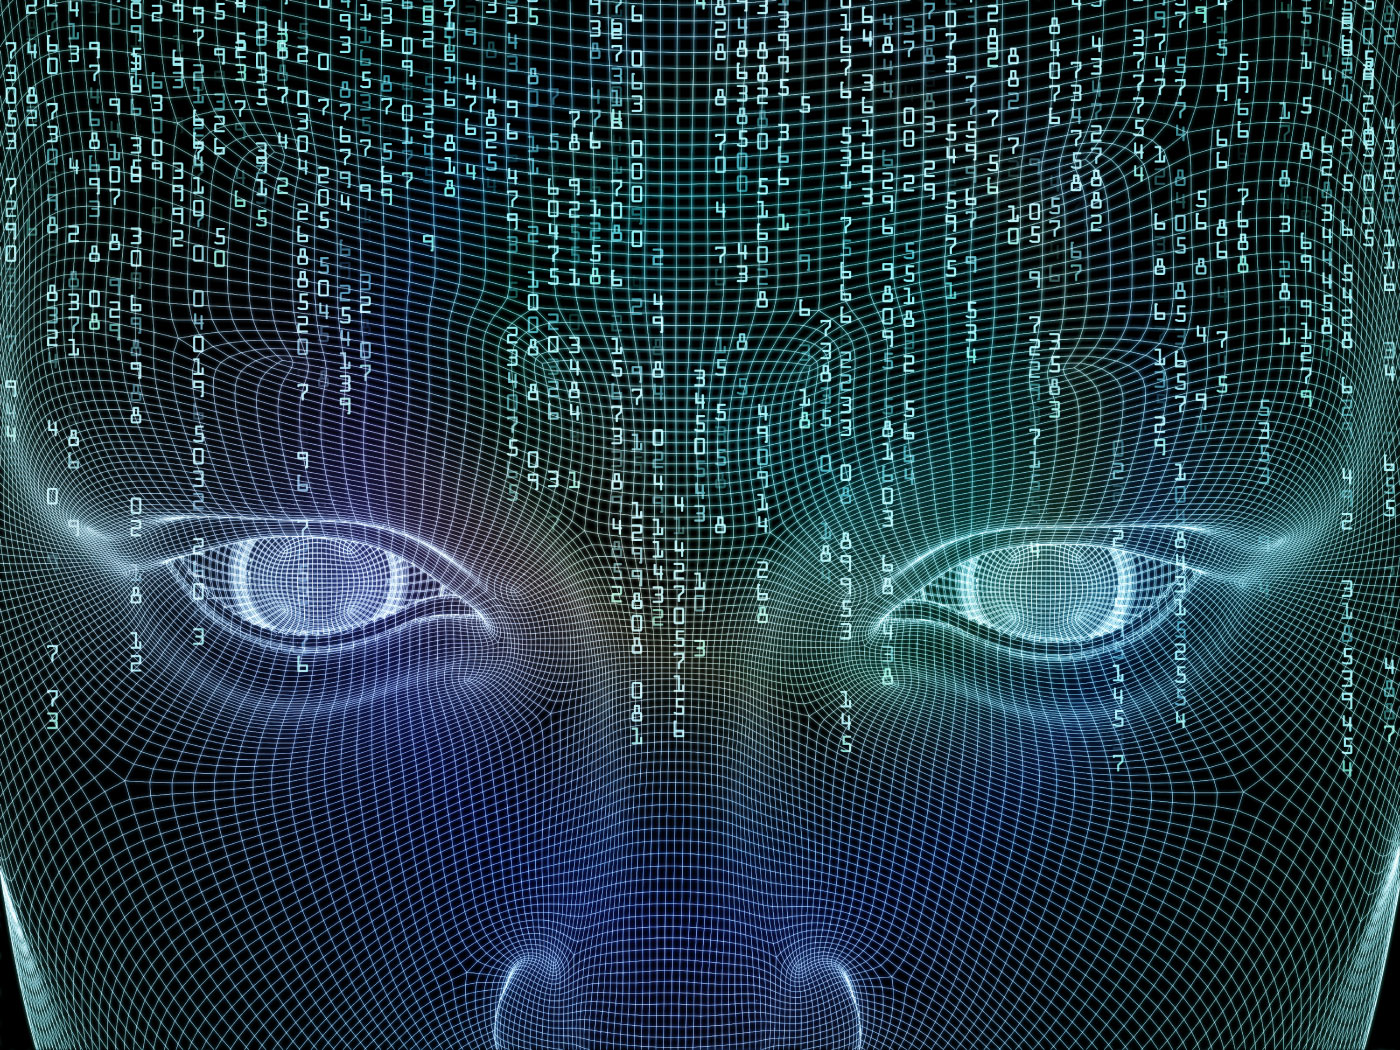
\includegraphics[width=\paperwidth]{pic/bkg}};}
\usepackage{tikz}

\DeclareGraphicsExtensions{.pdf,.png,.jpg,.svg}


\setbeamertemplate{itemize items}[square]
\setbeamertemplate{enumerate items}[square]

\definecolor{Red}{RGB}{190,0,0}
\definecolor{Blue}{RGB}{0,0,190}
\setbeamertemplate{headline}{}



\title[HBT]{ Particle physics seminar \vspace{0.4cm}\\ Three particle Bose-Einstein correlation}
\author[Attila Bagoly]{\Large{Attila Bagoly}\\ \vspace{0.1cm}}
\date[\today]{\today}
\institute[ELTE]{
\large{Supervisor: Máté Csanád}
}

\begin{document}

\begin{frame}
  \titlepage
\end{frame}

\section{HBT}
\begin{frame}
\frametitle{HBT}
\begin{itemize}
\setlength{\itemsep}{8pt}
\item 1956. Robert Hanbury Brown and Richard Q. Twiss: A test of a new
type of stellar interferometer on Sirius
\item Two photomultiplier, different distances $\Rightarrow$ correlation in two measured intensity distributions
\item Measured correlation as function of detector distance $\rightarrow$ radius of Sirius
\end{itemize}
\begin{figure}
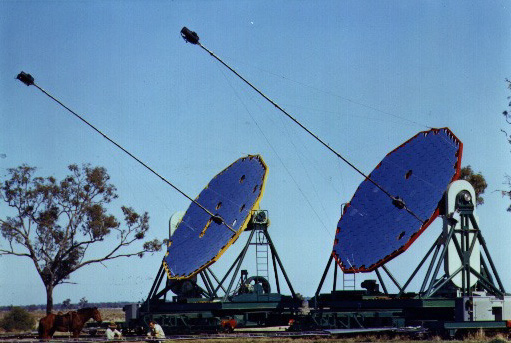
\includegraphics[scale=0.4]{pic/hbtdet.jpg}
\end{figure}
\end{frame}

\section{HBT in particle physics}
\begin{frame}
\frametitle{HBT in particle physics}
\begin{itemize}
\setlength{\itemsep}{14pt}
\item  1959. G. Goldhaber, S. Goldhaber, W.Y. Lee and A. Pais:
proton-antiproton collisions at 1.05 GeV/c:\vspace*{0.2cm}
\begin{itemize}
\setlength{\itemsep}{10pt}
\item investigating $\rho^0\rightarrow \pi^+\pi^-$ decay
\item unexpected correlation between $\pi^+$ and $\pi^+$, $\pi^-$ and $\pi^-$
\item 1960: reason pions are bosons
\end{itemize}
\item Latter was found out correlations contain info about geometry of source
\end{itemize}
\end{frame}

\begin{frame}
\frametitle{HBT in particle physics}
\begin{itemize}
 \item Amplitude:
 \vspace*{-10pt}
\begin{align*}
A(k_1, k_2) =  \frac{1}{\sqrt{2}}\bigg(e^{-ik_1(x_A-x_1)+i\Phi_1}e^{-ik_2(x_B-x_2)+i\Phi_2}\\\pm e^{-ik_1(x_A-x_2)+i\phi_2'}e^{-ik_2(x_B-x_1)+i\Phi_1'}\bigg)
\end{align*}
\end{itemize}

\begin{minipage}[b]{0.49\textwidth}
\begin{itemize}
\setlength{\itemsep}{8pt}
\item Probability of joint observation of the two particle with $k_1, k_2$ momentum:
\begin{align*}
P_2(k_1, k_2) = \langle |A(k_1, k_2)|^2 \rangle \\=1\pm \cos{(k_1-k_2)(x_1-x_2)}
\end{align*}
\item Chaotic emission: average over random phases $\rightarrow \Phi_i$ not present
\end{itemize}

\end{minipage}
\begin{minipage}[b]{0.49\textwidth}
\begin{figure}
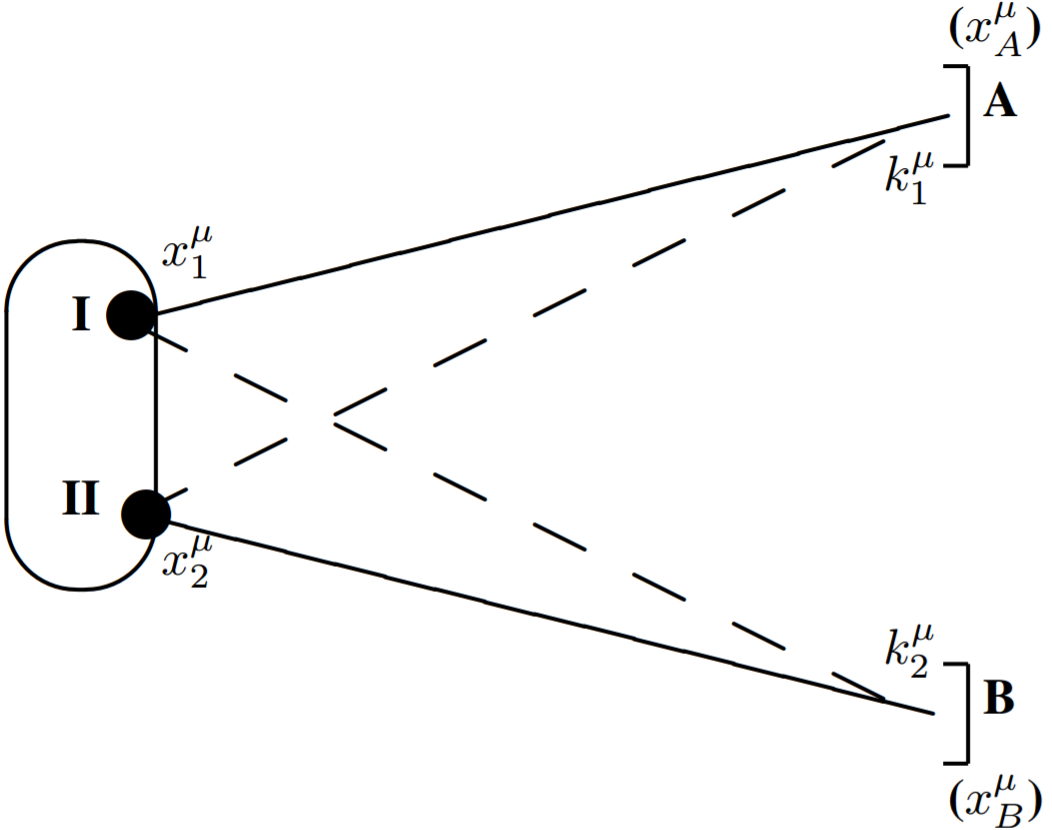
\includegraphics[scale=0.25]{pic/corr.png}
\end{figure}
\end{minipage}
\end{frame}

\begin{frame}
\frametitle{HBT in particle physics}
\begin{itemize}
\setlength{\itemsep}{8pt}
\item Single particle amplitude:
\begin{equation*}
A(k_i) = \frac{1}{\sqrt{2}}\bigg(e^{-ik_i(x_A-x_1)+i\Phi_1}\pm e^{-ik_i(x_A-x_2)+i\Phi_2}\bigg)
\end{equation*}
\item One particle probability distribution:
\begin{equation*}
P_1(k_i) = \langle |A(k_i)|^2 \rangle = 1
\end{equation*}
\item Two particle correlation:
\begin{equation*}
C_2(k_1, k_2) = \frac{P_2(k_1, k_2)}{P_1(k_1)P_1(k_2)} = 1\pm \cos{(k_1-k_2)(x_1-x_2)}
\end{equation*}
\end{itemize}
\end{frame}


\begin{frame}
\frametitle{HBT in particle physics}
\begin{itemize}
\setlength{\itemsep}{8pt}
\item More generally, for extended sources ($\rho(x)$ normalized space-time distribution):
\begin{align*}
P_2(k_1, k_2) = P_1(k_1)P_1(k_2)\int d^4x_1d^4x_2 |A(k_1, k_2)|^2\rho(x_1)\rho(x_2)\\=P_1(k_1)P_1(k_2)\big[1\pm |\tilde{\rho}(q)|^2\big]
\end{align*}
\item $q^\mu=k_1^\mu-k_2^\mu$ and
\begin{equation*}
\tilde{\rho}(q)=\int d^4x e^{iq^\mu x_\mu}\rho(x)
\end{equation*}
\item Correlation function:
\begin{equation*}
C_2(k_1, k_2) = \frac{P_2(k_1, k_2)}{P_1(k_1)P_1(k_2)} = 1\pm |\tilde{\rho}(q)|^2
\end{equation*}
\item Correlation function $\rightarrow$ Fourier transform $\rightarrow$ Source function
\end{itemize}
\end{frame}


\begin{frame}
\frametitle{Three particle HBT}
\begin{itemize}
\setlength{\itemsep}{8pt}
\item Invariant momentum distributions: $N_1(p_i), N_2(p_1,p_2),N_3(p_1, p_2, p_3)$
\item The definition of the correlation function:
\begin{equation*}
C_n(p_1,\dots,p_n)=\frac{N_n(p_1,\dots,p_n)}{N_1(p_1)\cdots N_1(p_n)}
\end{equation*}
 for chaotic emission:
\begin{equation*}
N_n(p_1,\dots,p_n)=\int \prod_{i=1}^{n}\mathcal{S}(x_i,p_i)|\Psi_{n}(\{x_i\})|^2 d^4x_1\dots d^4x_n
\end{equation*}
\item $\mathcal{S}(x,p)$ source function (usually assumed to be Gaussian - Levy is more general)
\end{itemize}
\end{frame}

\begin{frame}
\frametitle{Core-Halo}
\begin{itemize}
\setlength{\itemsep}{8pt}
\item Not all particles comes from QGP freeze out
\item they also can come from decays
\item Both part contribute to source function:
\begin{equation*}
\mathcal{S}=\mathcal{S}_{\rm core}+\mathcal{S}_{\rm halo}
\end{equation*}
\item Particle distribution:
\begin{equation*}
N_n(p_1,\dots,p_n) = N_n^{c}(p_1,\dots,p_n)+N_n^{h}(p_1,\dots,p_n)
\end{equation*}
\item Two particle correlation:
\begin{equation*}
C_2(k_1, k_2) =  1+\lambda_2|\mathcal{S}(q)|^2
\end{equation*}
where
\begin{equation*}
\sqrt{\lambda_2} =  f_C \equiv \frac{N^c}{N^c+N^h} 
\end{equation*}
\end{itemize}
\end{frame}

\begin{frame}
\frametitle{Coherence}
\begin{itemize}
\setlength{\itemsep}{8pt}
\item If the core partially emits particles in coherent manner:
\begin{equation*}
\mathcal{S}_{\rm core}=\mathcal{S}_{\rm core}^{\rm pc}+\mathcal{S}_{\rm core}^{i}
\end{equation*}
where pc refers to partially coherent, i to incoherent
\item Particle distribution:
\begin{equation*}
N_n^{c}(p_1,\dots,p_n) = N_n^{c,{\rm pc}}(p_1,\dots,p_n)+N_n^{c, {\rm i}}(p_1,\dots,p_n)
\end{equation*}
\item Two particle correlation: $C_2(k_1, k_2) =  1+\lambda_2|\mathcal{S}(q)|^2$, but $\lambda_2 \neq f_C^2$
\item Fraction of coherently produced pions:
\begin{equation*}
p_C \equiv \frac{N_{\rm coherent}}{N^{\rm coherent}+N^{\rm incoherent}} \rightarrow \lambda_2(f_C, p_C)
\end{equation*}
\item Can this happen? Yes,  e.g. due to formation of pion laser or Bose-Einstein condensate of pions
\end{itemize}

\end{frame}

\section{Motivation}
\begin{frame}
\frametitle{Motivation behind three particle HBT analysis}
\begin{itemize}
\setlength{\itemsep}{10pt}
\item Reminder: $C_2(k) = 1 + \lambda_2 |\mathcal{S}(q)|^2$
\item Two particle correlation strength: $\lambda_2 \equiv C_2(q=0)-1$
\item Similar definition of three particle correlation strength: $\lambda_3 \equiv C_3(0)-1$
\item Core-Halo: \vspace*{-15pt}
	\begin{align*}
		\lambda_2=f_C^2,\;\;\;\;\lambda_3 = 2f_C^3+3f_C^2 \\ 
		\kappa_3=\big(\lambda_3-3\lambda_2\big)/\big(2\sqrt{\lambda_2^3}\big)=1
	\end{align*}
\item Partial coherence ($p_C$ fraction of coherently produced $\pi$): 
	\begin{gather*}
		\lambda_2=f_C^2\big[(1-p_C)^2+2p_C(1-p_C)\big]\\
		\lambda_3=2f_C^3\big[(1-p_C)^3+3p_C(1-p_C)^2\big]+3f_C^2\big[(1-p_C)^2+2p_C(1-p_C)\big]\nonumber\\
		\kappa_3 = \kappa_3(p_C)
	\end{gather*}
\item From $\lambda_2$, $\lambda_3$ we can investigate the deviation from simple Core-Halo
\end{itemize}
\end{frame}

\section{Dimension}
\begin{frame}
\frametitle{Dimension}
\begin{itemize}
\setlength{\itemsep}{12pt}
\item Definition of correlation function:
\begin{equation}
C_3(\bm{k_1}, \bm{k_2}, \bm{k_3})=\frac{N_3(\bm{k_1}, \bm{k_2}, \bm{k_3})}{N_1(\bm{k_1})N_1(\bm{k_2})N_1(\bm{k_3})}\;\;\;\;\;\; \mathrm{(9D)} \label{eq:e1}
\end{equation}
\item Transverse momentum:
\begin{equation}
p_T=\big|\bm{p}_{T1}+\bm{p}_{T2}+\bm{p}_{T3}\big|/3
\end{equation}
\item Momentum differences: $\bm{k_{ij}}=\bm{k_i}-\bm{k_j}$
\item So we want to measure $C_3(\bm{k_{12}}, \bm{k_{13}}, \bm{k_{23}})$ for different $p_T$ bins (6D)
\end{itemize}
\end{frame}


\begin{frame}
\frametitle{Correlation function}
\begin{itemize}
\setlength{\itemsep}{14pt}
\item We use side-out-longitudinal decomposition:
\begin{itemize}
\setlength{\itemsep}{6pt}
\item long direction: beam direction
\item out direction: direction of average transverse momentum
\item side: orthogonal to long and out
\end{itemize}
\item Coordinate system: LCMS (longitudinal co-moving system) of the triplet: Lorentz boost in long direction
\item Instead of $\bm{k_{ij}^{\mathrm{LCMS}}}$ we measure correlation as function of 
\begin{equation*}
k_{ij}=|\bm{k_{ij}^{\mathrm{LCMS3}}}|\;\;\;\;\;\;\;\;\;\;\;\;\;(3D)
\end{equation*}
\item Reason: not enough statistics
\end{itemize}
\end{frame}

\section{What and how we measure}
\begin{frame}
\frametitle{Details of measurement}
\begin{itemize}
\setlength{\itemsep}{22pt}
\item BNL RHIC, PHENIX experiment, 200GeV Au+Au collision
\item Event-mixing method to measure correlation
\item Momentum difference distributions of pion pairs within the triplet from same event: $A(k_{12}, k_{13}, k_{23})$
\item Background distribution (triplets from different events): $B(k_{12}, k_{13}, k_{23})$
\item MinBias: no centrality filtering
\item Lot of cuts (single track, matching cuts, pair cuts)
\end{itemize}
\end{frame}

\begin{frame}
\frametitle{Details of measurement}
\begin{itemize}
\setlength{\itemsep}{16pt}
\item Low bin behavior:
\begin{equation}
k_{ij}\rightarrow 0 \;\;\xRightarrow{\;\;\;?\;\;\;\;}\;\; A,B\rightarrow 0
\end{equation}
\begin{figure}
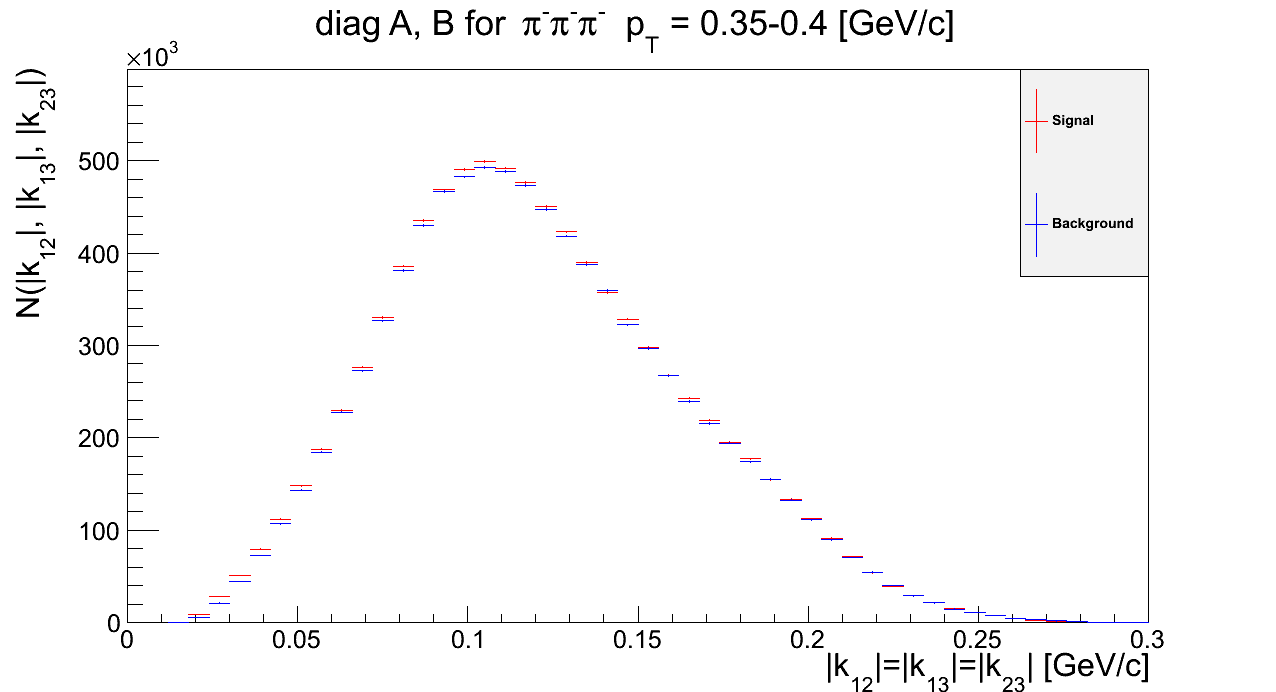
\includegraphics[scale=0.25]{pic/AB2}
\end{figure}
\end{itemize}
\end{frame}

\begin{frame}
\frametitle{Details of measurement}
\begin{itemize}
\setlength{\itemsep}{16pt}
\item The correlation:
\begin{equation}
C_3(k_{12}, k_{13}, k_{23})=\frac{A(k_{12}, k_{13}, k_{23})}{B(k_{12}, k_{13}, k_{23})}\frac{\int B}{\int A}
\end{equation}
\item Triangle inequality for $\vec{k}_{12}$, $\vec{k}_{13}$, $\vec{k}_{23}$
\begin{figure}
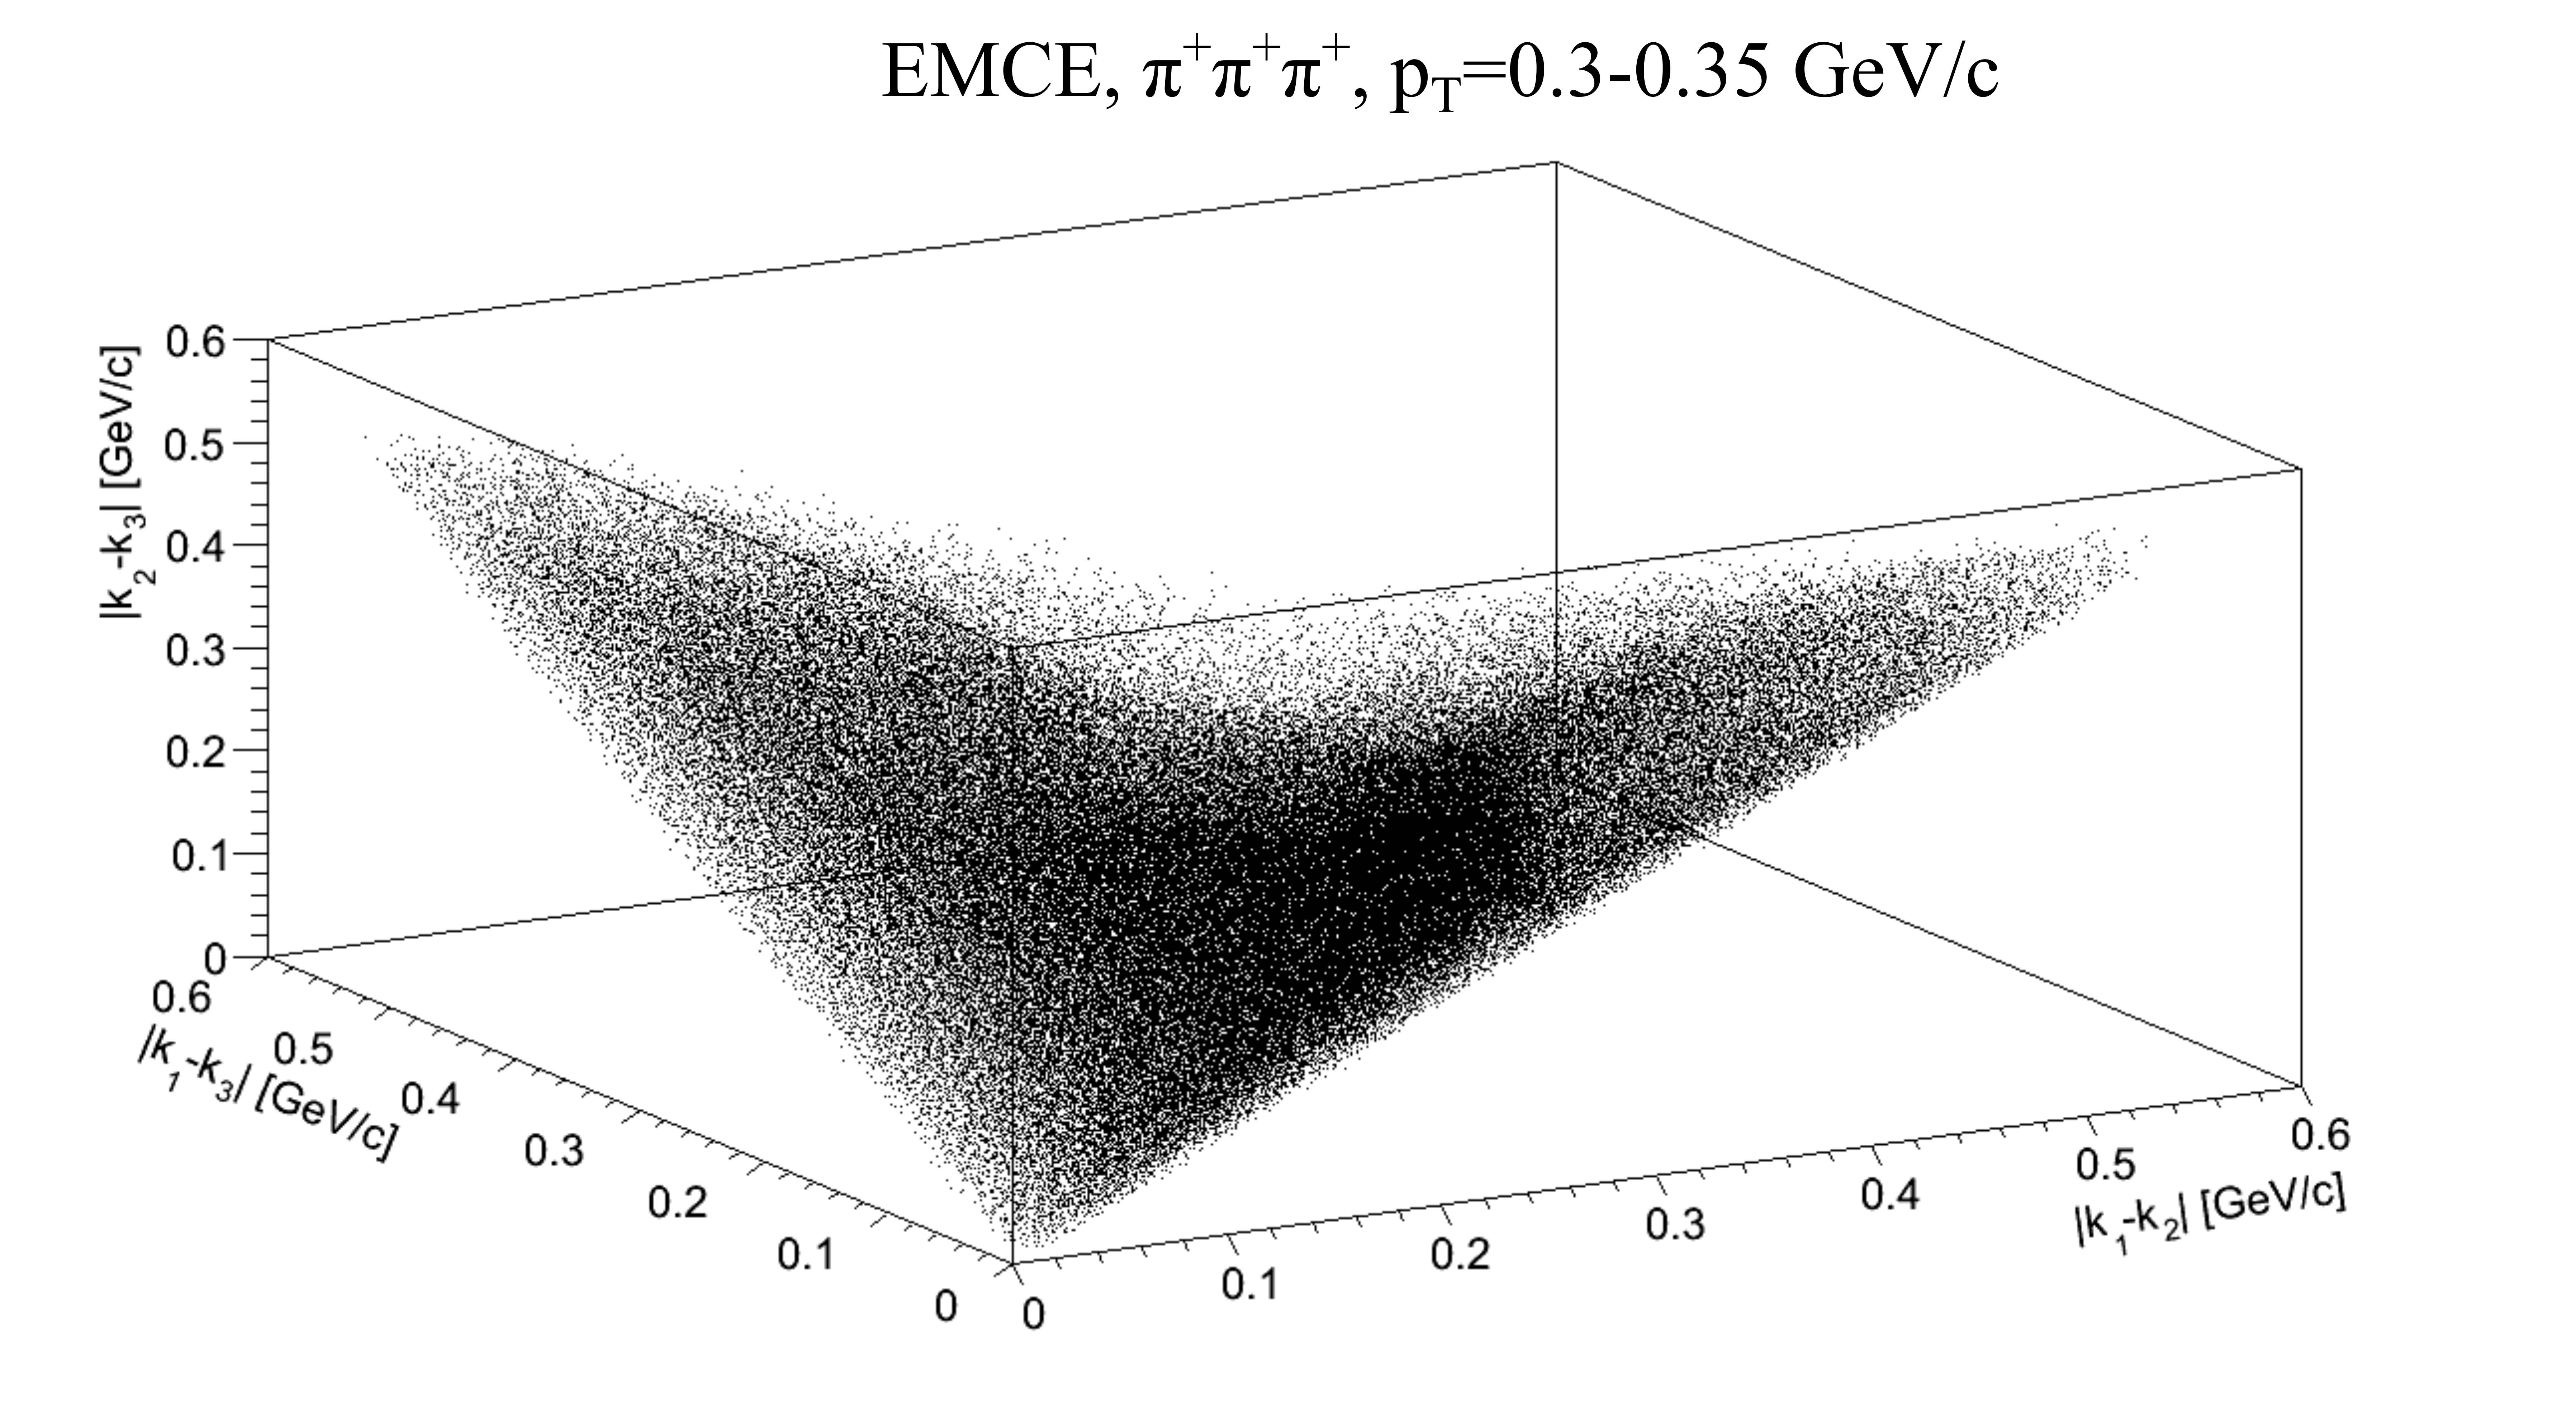
\includegraphics[scale=0.25]{pic/C1}
\end{figure}
\end{itemize}
\end{frame}

\begin{frame}
\frametitle{Details of measurement}
\begin{itemize}
\setlength{\itemsep}{16pt}
\item Order within triplet doesn't matter
\item But when we measure do matter $\Rightarrow$ we have to fold the histogram
		$A(5,6,7) \;+=\; A(6,7,5)\; + \;A(7,5,6)\; + \;A(5,7,6)\; $ $+ \;A(7,6,5)\;+\;A(6,5,7)$
\begin{figure}
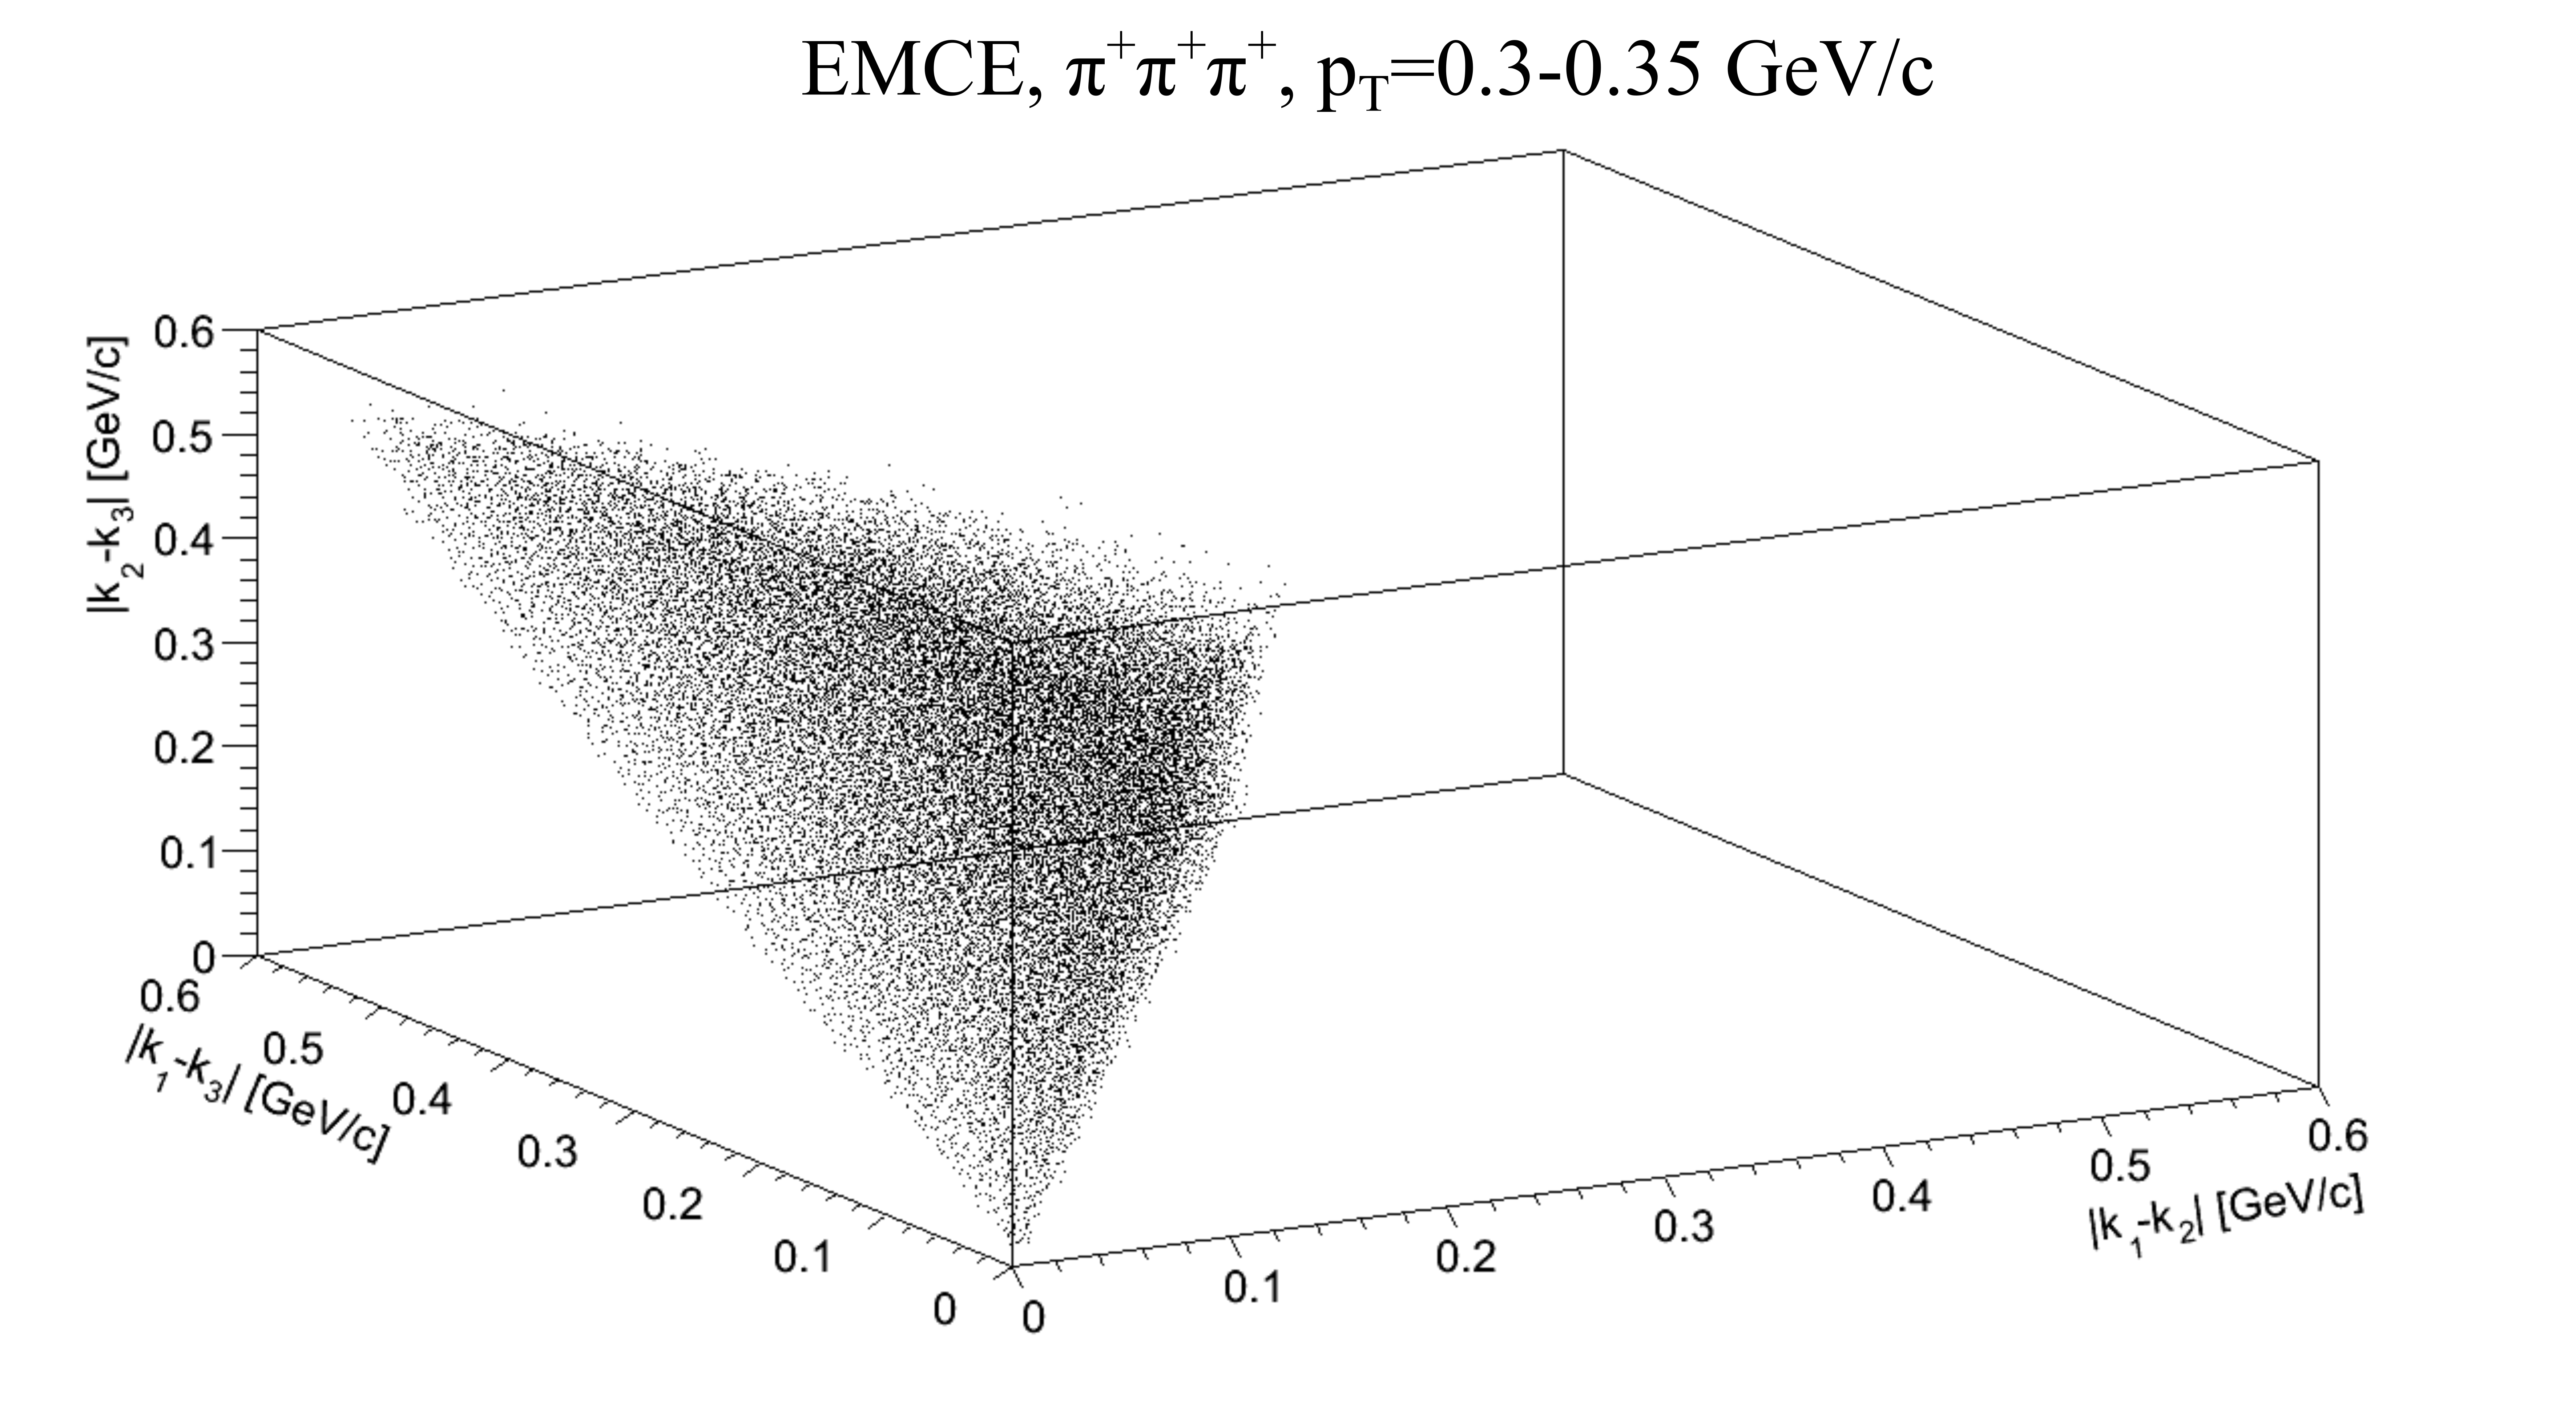
\includegraphics[scale=0.25]{pic/C2}
\end{figure}
\end{itemize}
\end{frame}

\begin{frame}
\frametitle{Details of measurement}
\begin{itemize}
\setlength{\itemsep}{16pt}
\item Diagonal correlation function
\end{itemize}
\begin{figure}
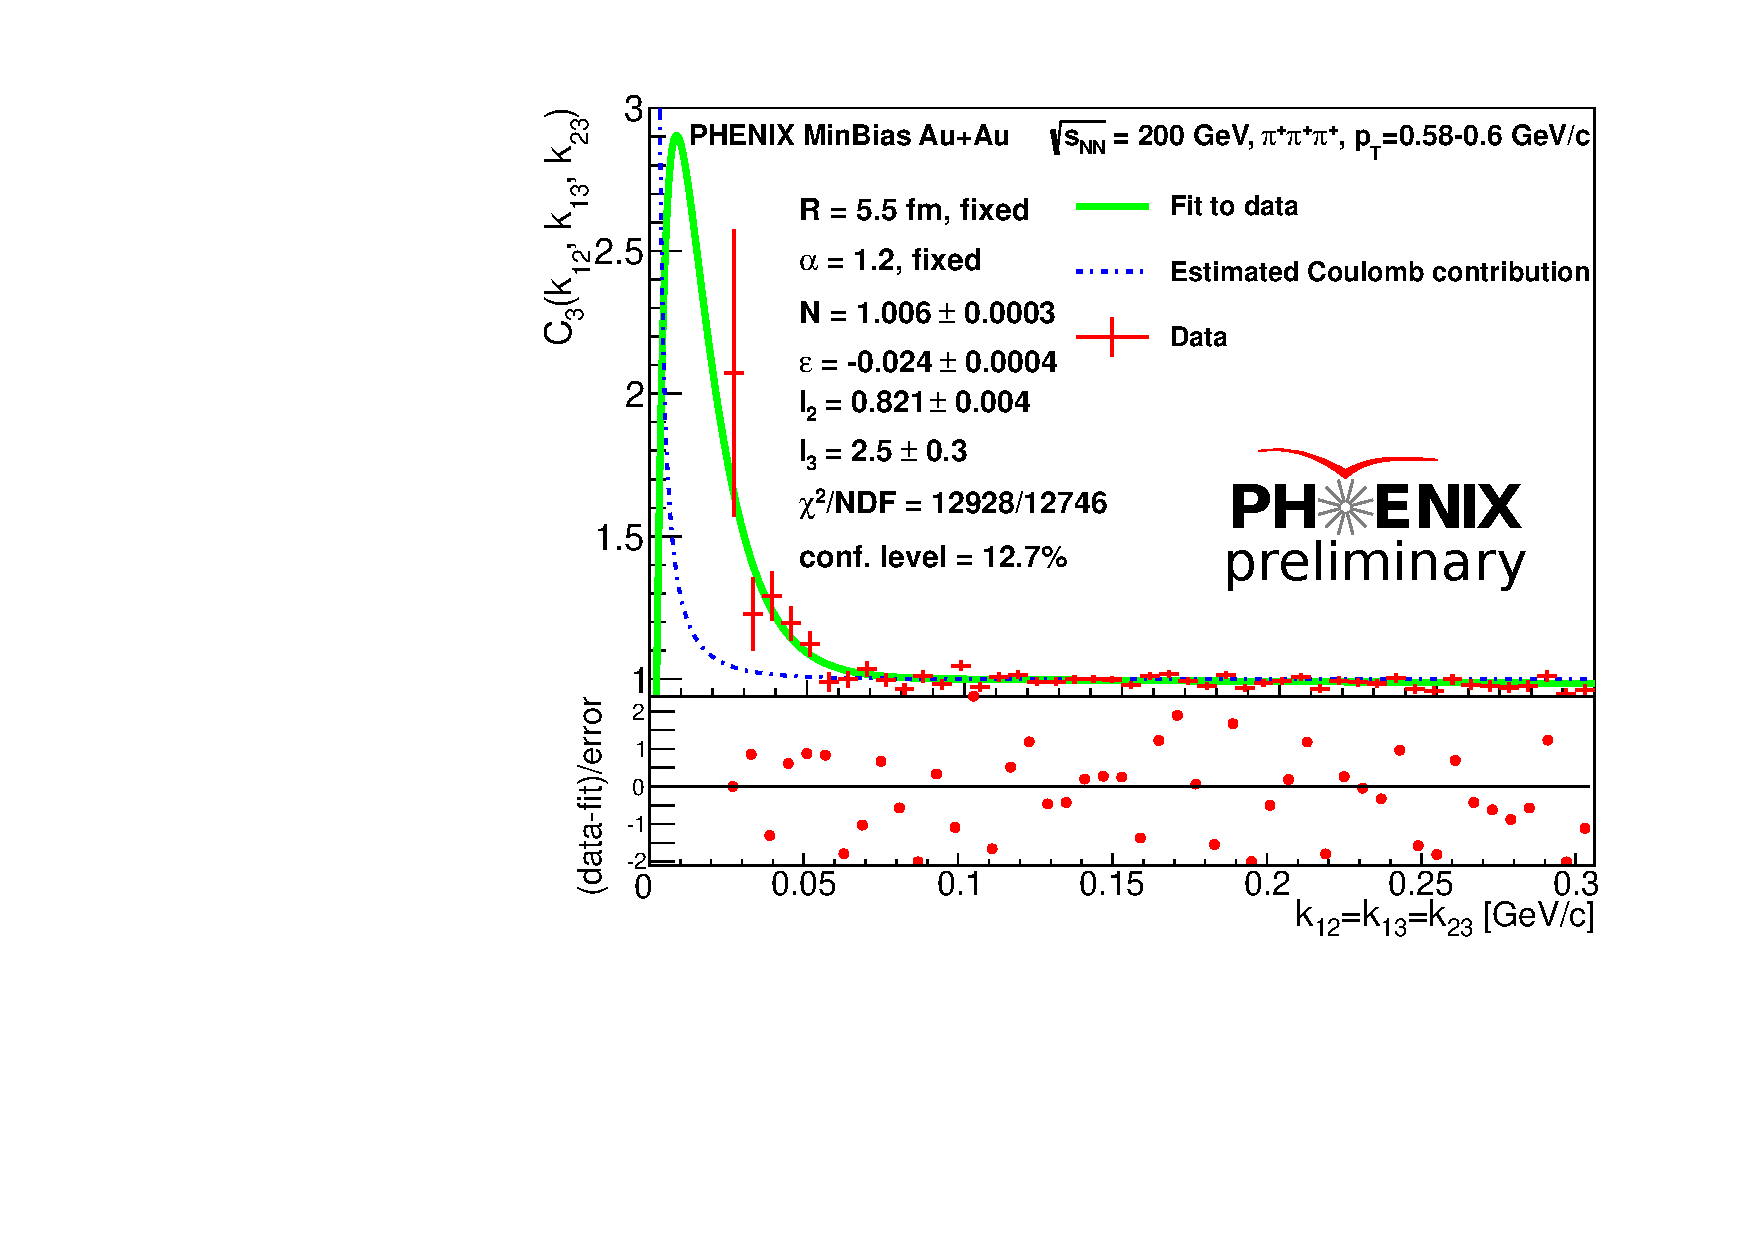
\includegraphics[scale=0.45]{pic/diag_highpt.pdf}
\end{figure}
\end{frame}

\section{Model}
\begin{frame}
\frametitle{Model without Coulomb correction}
\begin{itemize}
\setlength{\itemsep}{12pt}
\item Assumption for source: Levy-distribution
\begin{equation*}
\mathcal{L}(\alpha,R,r)=(2\pi)^{-3} \int d^3q e^{iqr} e^{-\frac{1}{2}|qR|^{\alpha}}
\end{equation*}
\item Approximation for $C_3$ can be derived ($\mathcal{L}_3=2f_C^3$):
\begin{align*}
C_3^{(0)}(k_{12}, k_{13}, k_{23}) = 1+ \ell_3e^{-0.5(|2k_{12}R_C|^\alpha+|2k_{13}R_C|^\alpha+|2k_{23}R_C|^\alpha)}\nonumber\\
+\ell_2\bigg(e^{|2k_{12}R_C|^\alpha}+e^{|2k_{13}R_C|^\alpha}+e^{|2k_{23}R_C|^\alpha}\bigg)
\end{align*}
\item Background: $N(1+\epsilon k_{12})(1+\epsilon k_{13})(1+\epsilon k_{23})$
\item Fit parameters: $\ell_3$, $\ell_2$,  $R_C$, $\alpha$, $N$, $\epsilon$
\item We are looking for: $\lambda_3 \equiv  C_3(k_{12}=k_{13}=k_{23}=0)-1=\ell_3+3\ell_2$
\item In an other analysis $\lambda_2$ was measured
\end{itemize}
\end{frame}

\begin{frame}
\frametitle{Coulomb correction}
\begin{itemize}
\setlength{\itemsep}{16pt}
\item Corrected model:
\begin{equation*}
C_3(k_{12}, k_{13}, k_{23}) = C_3^{(0)}(k_{12}, k_{13}, k_{23})\cdot K_3(k_{12}, k_{13}, k_{23})
\end{equation*}
\item ''Generalized Riverside'' method for 3 particle Coulomb problem
\begin{equation*}
K_3(k_{12}, k_{13}, k_{23}) \approx K_1(k_{12})K_1(k_{13})K_1(k_{23})
\end{equation*}
\end{itemize}
\begin{figure}
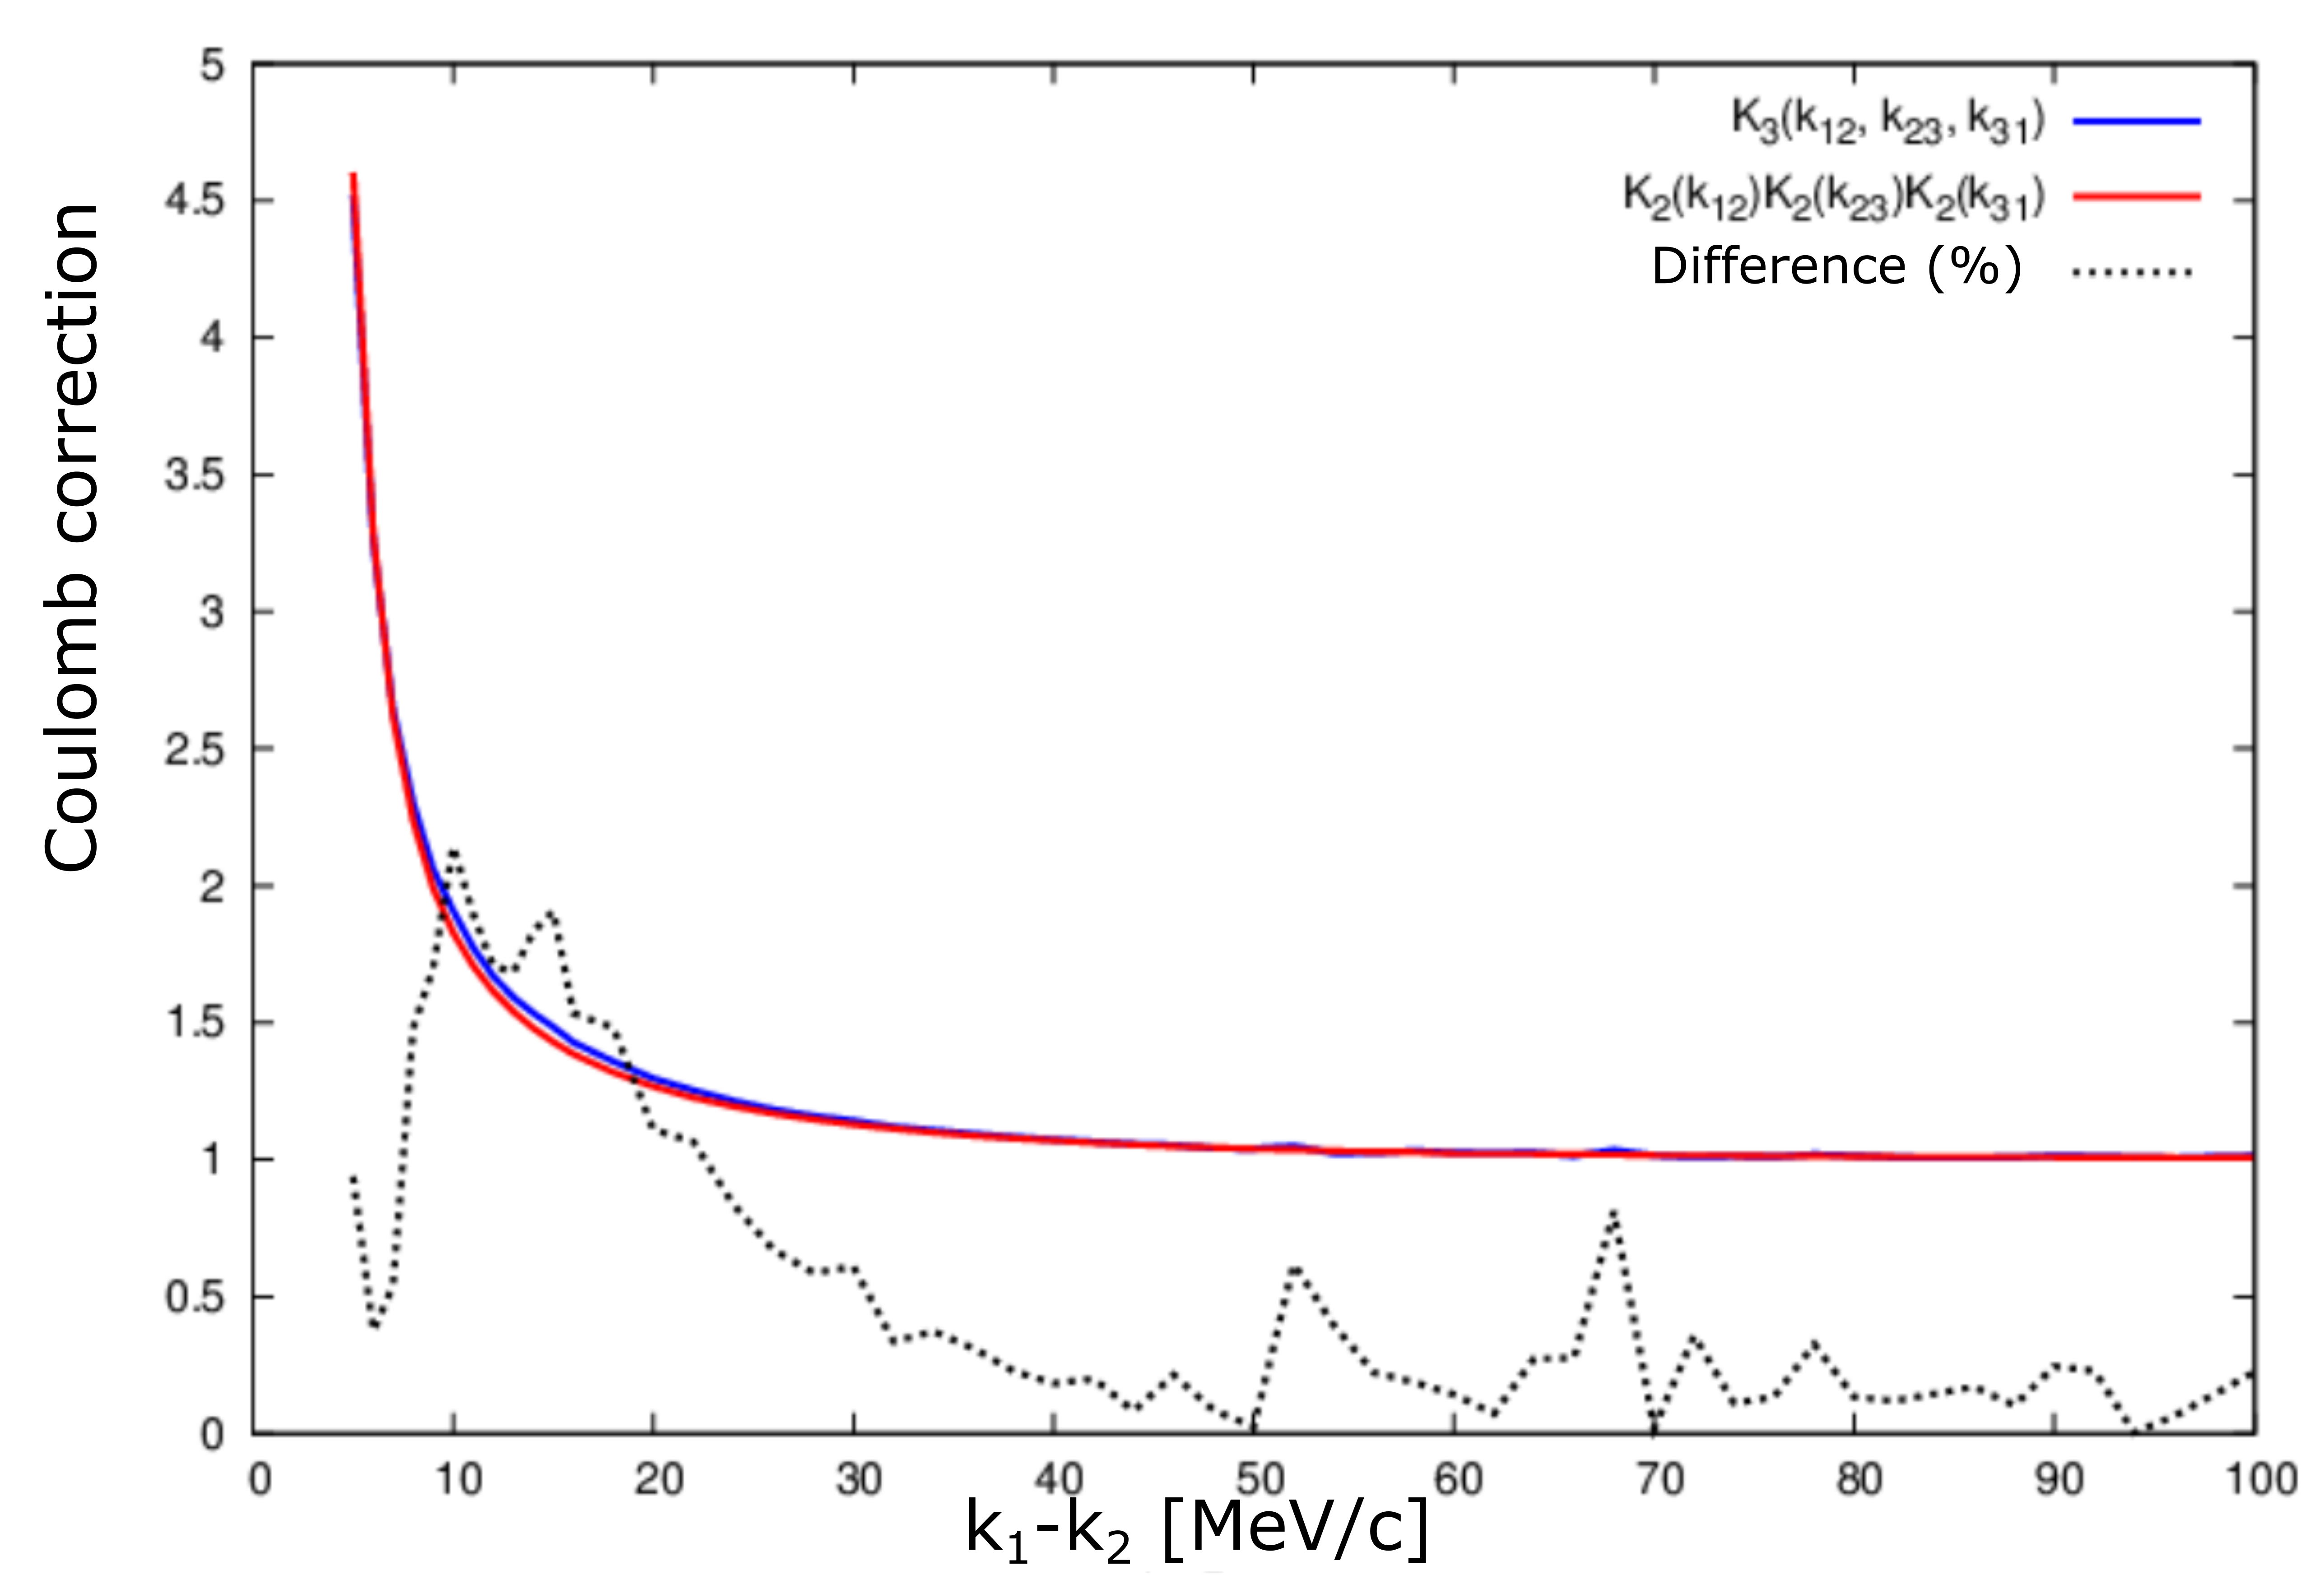
\includegraphics[scale=0.25]{pic/coulomb1}
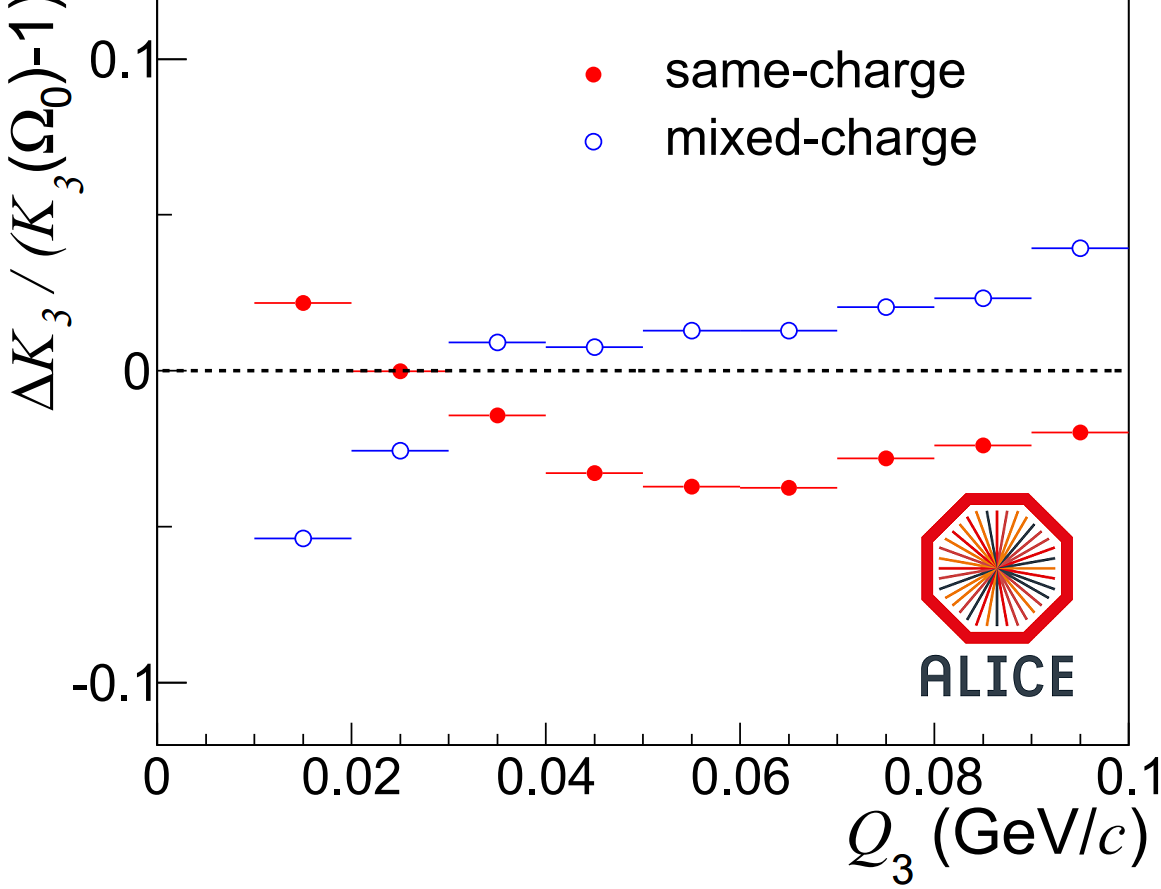
\includegraphics[scale=0.235]{pic/coulomb2}
\end{figure}
\end{frame}

\begin{frame}
\frametitle{Three particle correlation strength: $\lambda_3$}
\begin{itemize}
\setlength{\itemsep}{10pt}
\item $\lambda_3$ within Core-Halo  + chaotic emission range for all $m_T$
\end{itemize}
\begin{figure}
\colorbox{white}{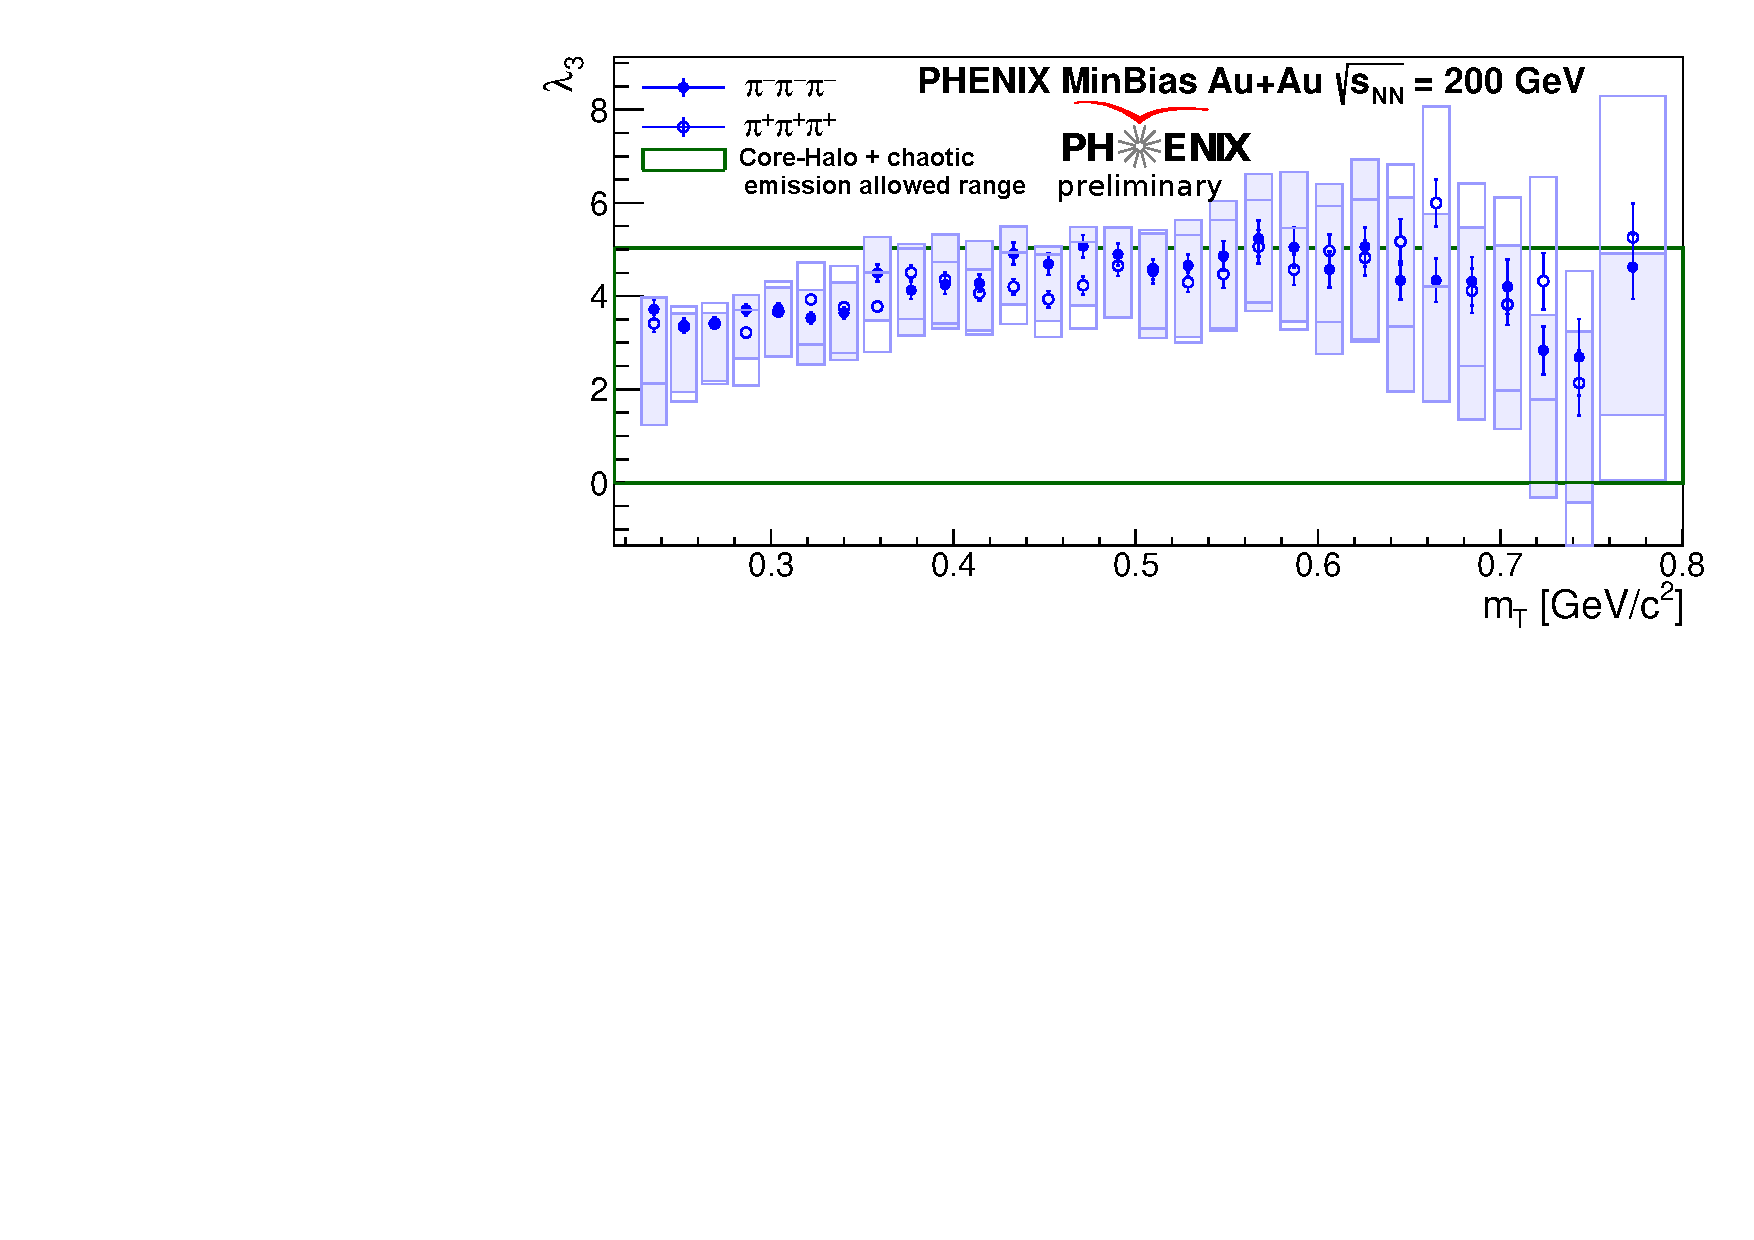
\includegraphics[scale=0.6]{pic/lambda3}}
\end{figure}
\end{frame}



\begin{frame}
\frametitle{Core-Halo independent parameter}
\begin{itemize}
\item $\kappa_3\equiv\frac{\lambda_3-3\lambda_2}{2\sqrt{\lambda_2^3}}$ not depend on $f_C$ ($f_C=\mathrm{core}/(\mathrm{core}+\mathrm{halo})$)
\item Core-Halo + chaotic emission: $\kappa_3=1$
\item additional effect (eg. not fully thermal): $\kappa_3\neq 1$
\item Statistically significant deviation from $\kappa_3=1$
\end{itemize}
\begin{figure}
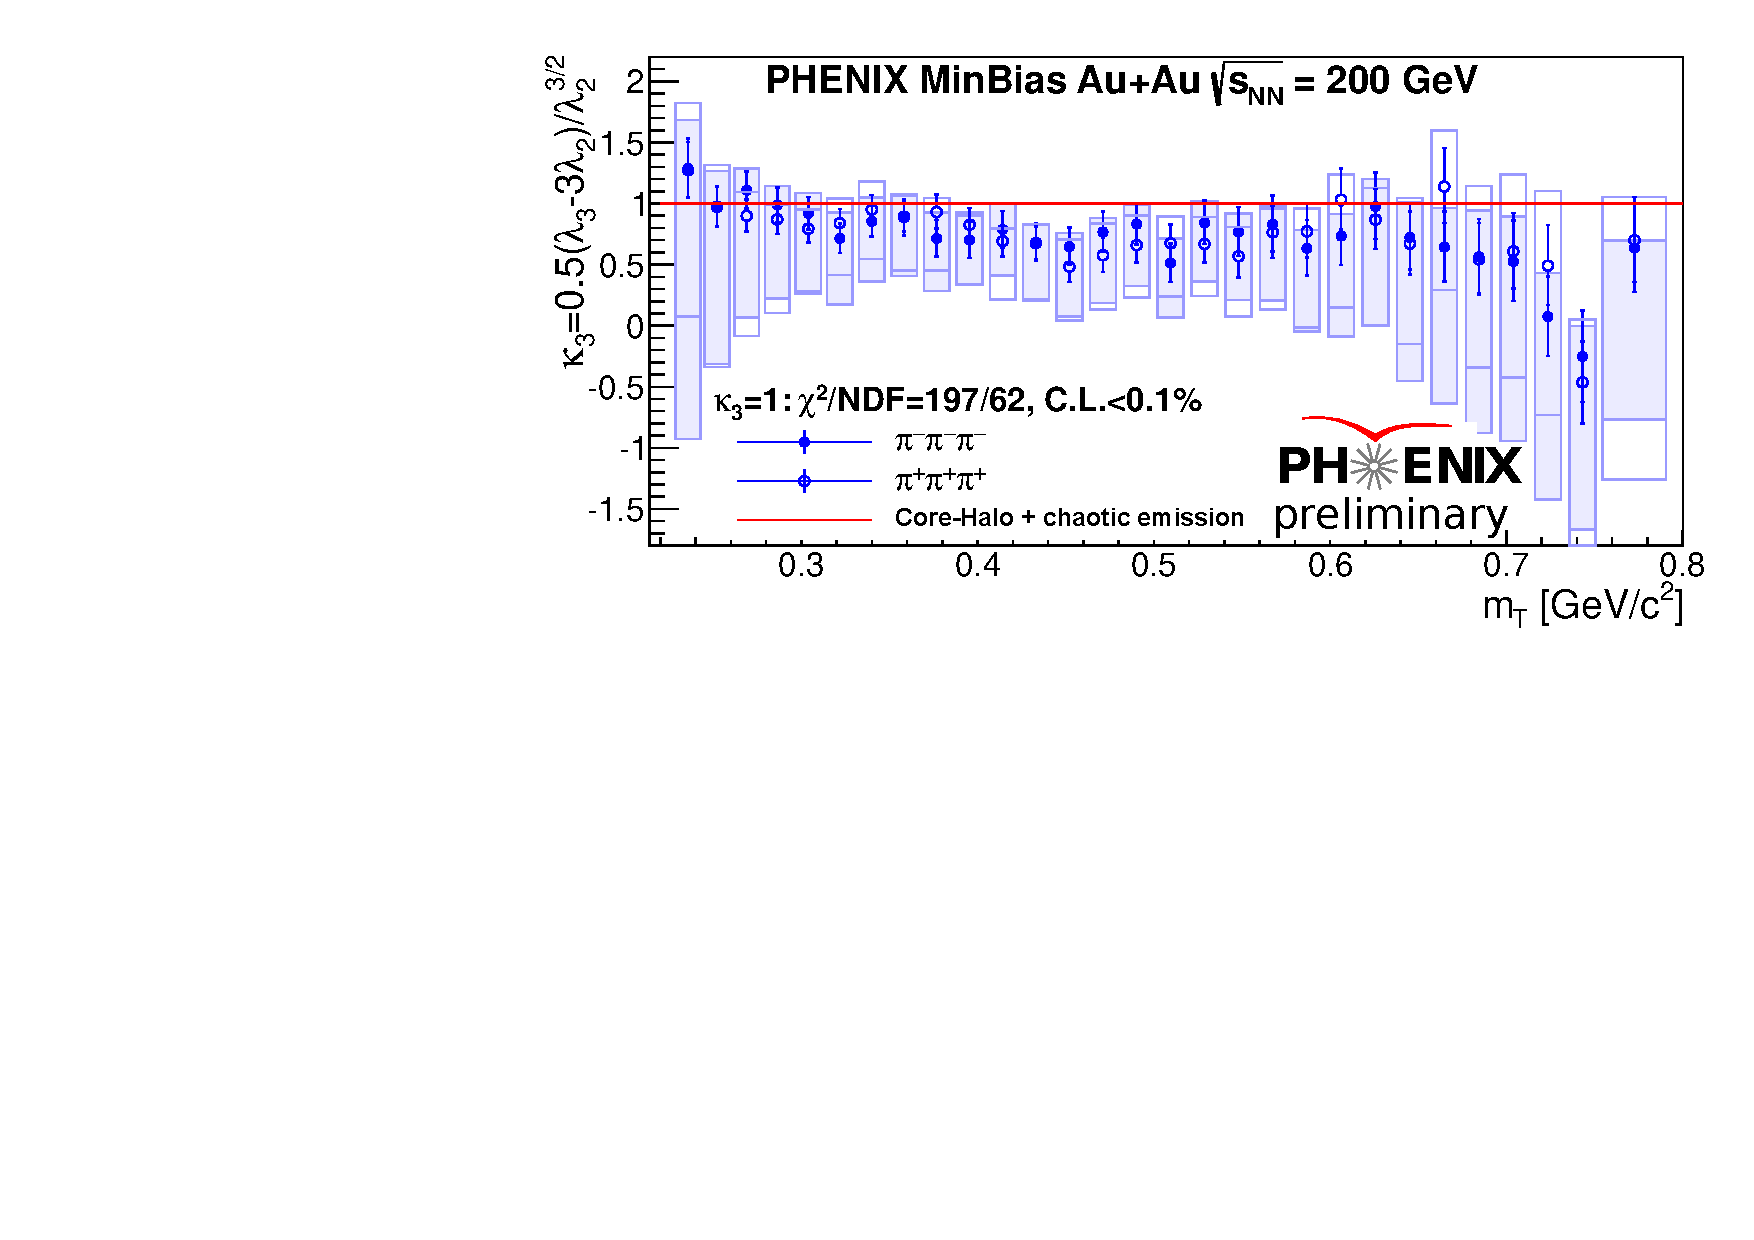
\includegraphics[scale=0.5]{pic/kappa3}
\end{figure}
\end{frame}


\begin{frame}
\frametitle{Partial coherence ($p_c$) vs fractional core}
\begin{itemize}
\vspace{-0.004\textheight}
\item Simple theoretical model: $\lambda_2(f_c, p_c)$, $\lambda_3(f_c, p_c)$ 
\item Measured $\lambda_2^{\rm meas.} \rightarrow \lambda_2^{\rm meas.}=\lambda_2(f_c,p_c) \Longrightarrow f_c(p_c)$ (green lines)
\item Measured $\lambda_3^{\rm meas.} \rightarrow \lambda_3^{\rm meas.}=\lambda_3(f_c,p_c) \Longrightarrow f_c(p_c)$ (blue lines)
\item $f_c<0.82$ and $p_c>0.5$ can be excluded, $p_C<0.5$ can't be excluded
\end{itemize}

\begin{figure}
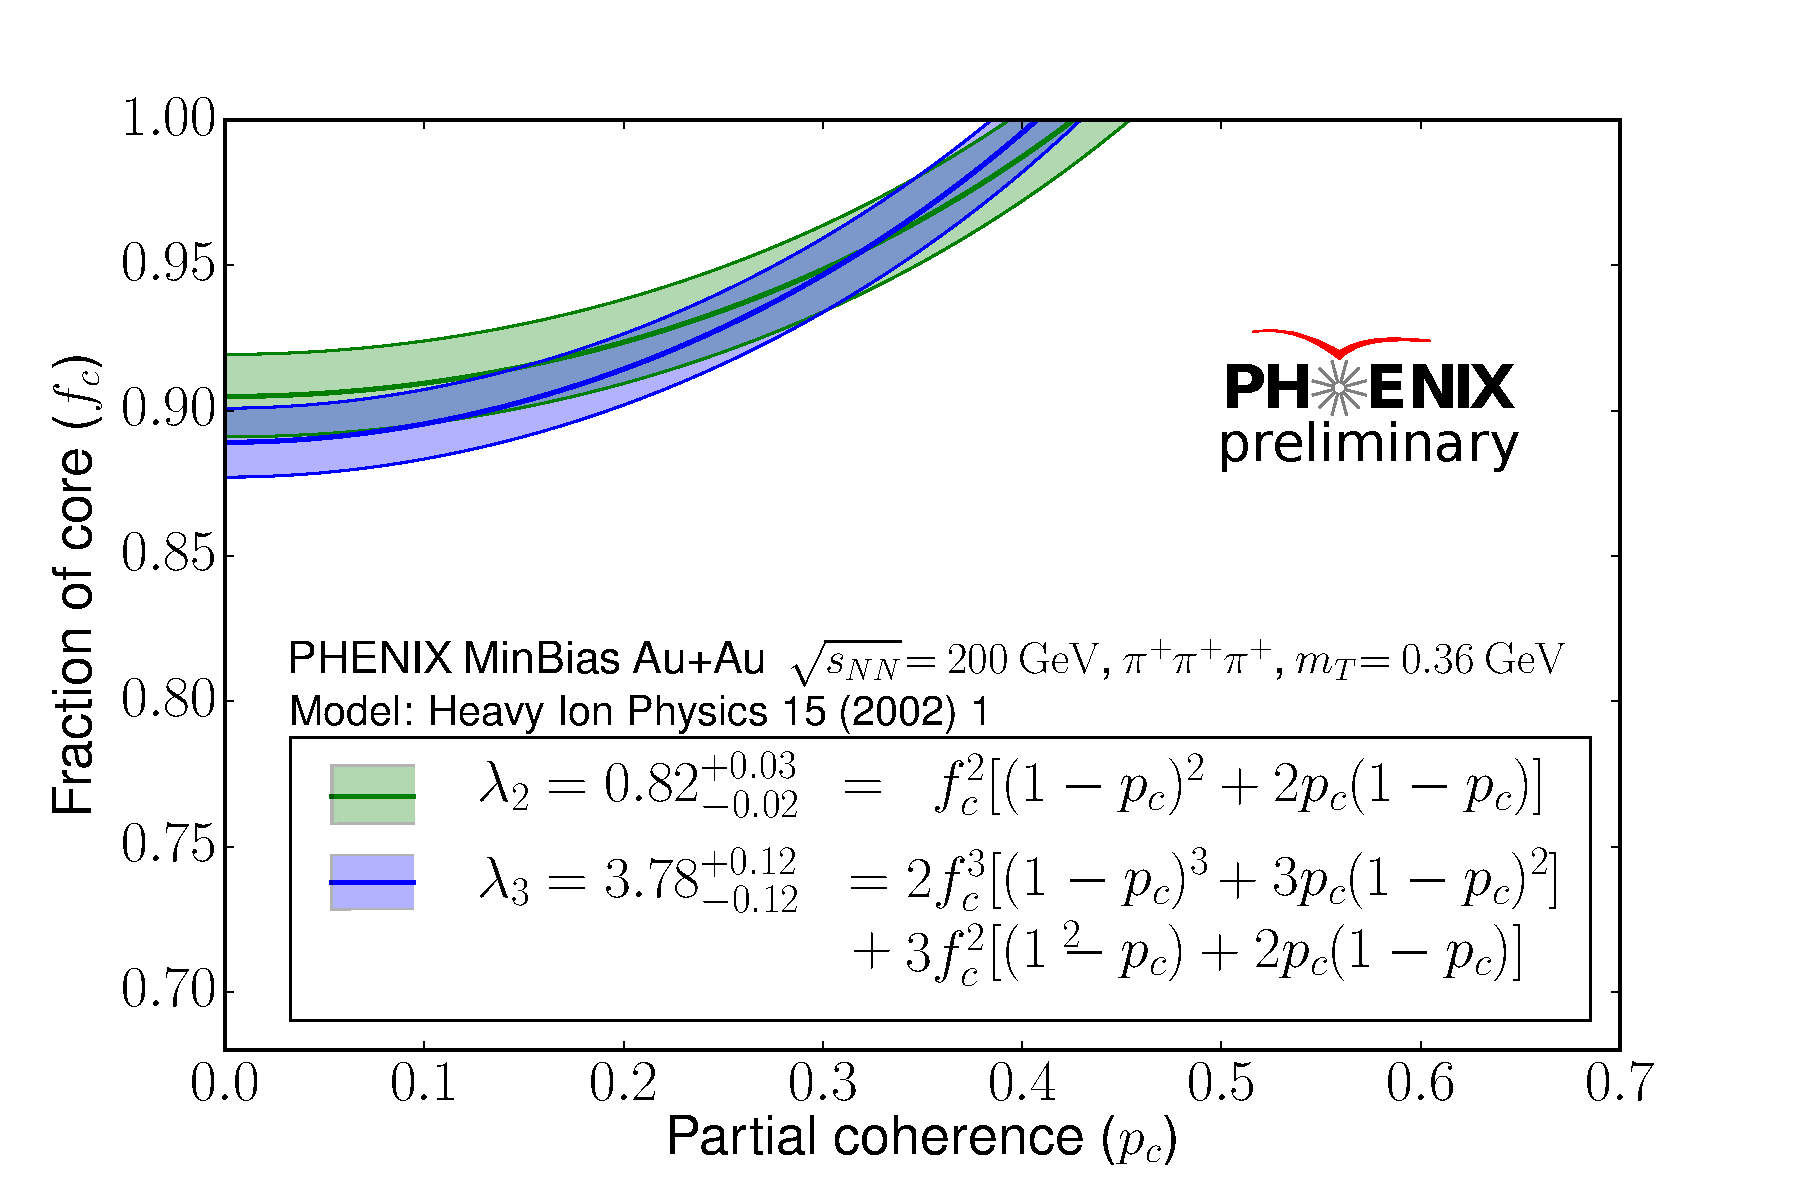
\includegraphics[width=0.7\textwidth]{pic/cropped_fcpc2}
\end{figure}
\end{frame}


\end{document}

